\documentclass[11pt]{article}
\usepackage[margin=1in]{geometry}          
\usepackage{graphicx}
\usepackage{amsthm, amsmath, amssymb}
\usepackage{setspace}\onehalfspacing
\usepackage[loose,nice]{units} %replace "nice" by "ugly" for units in upright fractions
\usepackage{longtable}

%Import the natbib package and sets a bibliography styles
\usepackage{natbib}
%\bibliographystyle{abbrvnat}
\bibliographystyle{unsrt} %numbers references in the order they appear in the text
%\setcitestyle{authoryear}
\setcitestyle{numbers,square}

\title{Reference sheet for {\it acpcdetect} version 2.1 usage}
\author{Babak A. Ardekani, PhD}
%\date{Spring 2015}

\begin{document}
\maketitle
\noindent {\large \bf Introduction:} 
The {\it acpcdetect} program is a module of the Automatic Registration Toolbox (ART). 
The program takes a 3D T1-weighted structural MRI of the human brain as input. 
It automatically detects the mid-sagittal plane (MSP) using the method described in \citep{pmid9533596}.
It then detects the AC and PC intersection points on the MSP using the method described in \citep{pmid19264138}. 
Finally, it detects 8 additional landmarks (the so-called Orion landmarks) on the MSP using the method 
described in \citep{pmid35288224}.  
This information is used to tilt-correct the input volume into a standard orientation.  
In this orientation: (1) the MSP is precisely aligned with the central plane of the FOV; 
(2) the anterior-posterior (AP) axis is on the MSP and aligned with the AC-PC line; 
(3) the inferior-superior (IS) axis is on the MSP and perpendicular to the AC-PC line; 
(4) the left-right (LR) axis is perpendicular to the MSP; and 
(5) the FOV center is approximately the mid-point between the AC and the PC on the MSP. 
The FOV center can alternatively be placed on the AC point using the -center-AC option.  
\vspace{3mm}

\noindent {\large \bf Installation on Linux and MacOS systems:}
A video demonstration of installing ART software can be found here:
https://www.youtube.com/watch?v=xCawMFQr50M\&t=26s \\
Althought I made this video for installing {\it atra}, a different module of ART, the steps are similar.

To install {\it acpcdetect}, you may need 
to be logged in as root, depending on the permissions of the directory in which
you are installing {\it acpcdetect}. Let's assume that {\it acpcdetect} will be installed in
/usr/local/art.
\begin{itemize}
\item[(a)] Set the ARTHOME environment variable to /usr/local/art. If ARTHOME is already
defined on your system, then you can skip this step. Otherwise, ``sh'' or ``bash'' users may define
ARTHOME using the following command: 

export ARTHOME=/usr/local/art 

To do this automatically at login, users should add the above line to their ``.bashrc'' or ``.profile''
file. Users of ``csh'' or ``tcsh'' may use the following command:

setenv ARTHOME /usr/local/art 

and add it to their ``.cshrc'' or ``.tcshrc'' file.

\item[(b)] Download the Linux or MacOS version of the software from www.nitrc.org/projects/art and
move it to \$ARTHOME.

\item[(c)] Unpack the package:

cd \$ARTHOME

tar -xvzf acpcdetect2.0*.tar.gz

\item[(d)] Move the executable program \$ARTHOME/bin/acpcdetect to a bin directory in your PATH, or
preferably, add the directory \$ARTHOME/bin to your PATH. This can be done by executing the
following command and adding it to the ``.bashrc'' file:

export PATH=\$ARTHOME/bin:\$PATH

\end{itemize}

\noindent {\large \bf Orientation code:} 
In ART, the anatomical orientation of 3D volumes is specified by a 3-letter orientation 
code consisting of a combination of letters A, P, L, R, S and I, denoting anterior, 
posterior, left, right, superior and inferior directions, respectively.  For example, 
the orientation code PIL indicates that the volume's $(i, j, k)$ voxel coordinates point 
towards posterior, inferior and left directions, respectively. Similarly, the orientation 
code RAS indicates that $(i, j, k)$ point to right, anterior and superior directions. 
There are 48 possible orientation codes. 
\vspace{3mm}

\noindent {\large \bf Usage:} 

acpcdetect [options] -i \textless input-volume\textgreater.nii
\vspace{3mm}

\noindent {\large \bf Required argument:}

\begin{longtable}{p{0.25\textwidth}p{0.68\textwidth}}
-i \textless input-volume\textgreater.nii &
3D T1-weighted MRI brain volume in NIFTI format of type short or unsigned short 
\end{longtable}

\noindent {\large \bf Options:}

\begin{longtable}{p{0.25\textwidth}p{0.68\textwidth}}
-v & Enables verbose mode \\

-lm \textless landmarks-file \textgreater &
A text file containing manually determined $(i, j, k)$ coordinates
of the AC, PC and VSPS (vertex of the superior pontine sulcus) landmarks in that order. 
When this file is supplied,
automatic detection of these landmarks is suppressed. This is useful
in cases when automatic landmark detection fails.\\

-no-tilt-correction & 
Does not tilt-correct the output, but the SFORM and QFORM are set
correctly in the output volume header. This is useful for applications
that would like to use {\it acpcdetect} as a preprocessing tilt-correction
step without applying interpolation at this stage.  \\ 

-center-AC &
Places the output volume's FOV center at AC \\

-standard &
Tilt-correction is performed without using the Orion landmarks.
Tilt-correction is done using the AC, PC and MSP only. This is the
method used in version 1.0 of {\it acpcdetect}.  In the current version 2.0, the
8 Orion landmarks are also used to stabilize the standardization of the
orientation. Using the -standard option, therefore, reverts back to the method
used by {\it acpcdetect} version 1.0 without using the additional Orion landmarks. \\

-output-orient \textless code\textgreater  &
Specifies the orientation of the output volume (default: RAS). 
In ART, orientation codes are 3-letter codes consisting of 6 letters:
A, P, I, S, L, R.  There are 48 possible combinations. For example
PIL for Posterior-Inferior-Left or RAS for Right-Anterior-Superior. \\

-nx \textless int\textgreater  &
	Number of voxels in $i$ direction (the fastest varying index) of the
	output volume. The default value is determined from the input volume. \\

-ny \textless int\textgreater  &
	Number of voxels in $j$ direction (the 2nd fastest varying index) of the
	output volume. The default value is determined from the input volume. \\

-nz \textless int\textgreater  &
	Number of voxels in $k$ direction (the slowest varying index) of the
	output volume. The default value is determined from the input volume. \\

-dx \textless float\textgreater &
	Voxel dimension of the output volume in $i$ direction. The default
	value is determined from the input volume. \\

-dy \textless float\textgreater &
	Voxel dimension of the output volume in $j$ direction. The default
	value is determined from the input volume. \\

-dz \textless float\textgreater &
	Voxel dimension of the output volume in $k$ direction. The default
	value is determined from the input volume. \\

-version &
	Prints software version \\

-help &
	Prints help information \\

-noppm &
	Prevents outputting *.ppm images \\

-nopng &
	Prevents outputting *.png images \\

-notxt &
	Prevents outputting *.txt files \\

-rvsps \textless r\textgreater  &
	Search radius for VSPS (default = 50 mm) \\

-rac \textless r\textgreater  &
	Search radius for AC (default = 15 mm) \\

-rpc \textless r\textgreater  &
	Search radius for PC (default = 15 mm) \\

-nn &
	Uses the nearest neighbor interpolation for tilt-correction 
\end{longtable}
\newpage

\noindent {\large \bf Output files:}

\begin{longtable}{p{0.4\textwidth}p{0.53\textwidth}}
\textless output-volume\textgreater.nii &
	The output volume is saved here. The default filename is
	\textless input-volume\textgreater\_RAS.nii. If a different orientation code is
specified using -output-orient, then this code replaces RAS in the output volume filename.
The output volume will be the tilt-corrected
	version of the input volume. However, if the -no-tilt-correction option is
	selected, the output volume will not be resliced (only reoriented). The
	tilt-correction information, however, are still written in the QFORM and
	SFORM entries of the image header as well as in the *.mrx and *.mat files
	(described below). \\

\textless input-volume\textgreater.mrx &
	Transformation matrix for tilt-correction in ART format \\

\textless input-volume\textgreater \_FSL.mat &
	Transformation matrix for tilt-correction in FSL format \\

\textless input-volume\textgreater \_ACPC\_sagittal.ppm &
	Sagittal view of the detected AC/PC locations in
	PPM format (output suppressed by -noppm option) \\

\textless input-volume\textgreater \_ACPC\_sagittal.png &
	Sagittal view of the detected AC/PC locations in
	PNG format (output suppressed by -nopng option) \\

\textless input-volume\textgreater \_ACPC\_axial.ppm &
	Axial view of the detected AC/PC locations in PPM
	format (output suppressed by -noppm option) \\

\textless input-volume\textgreater \_ACPC\_axial.png &
	Axial view of the detected AC/PC locations in PNG
	format (output suppressed by -nopng option) \\

\textless input-volume\textgreater \_orion.ppm &
	Mid-sagittal view of the detected Orion landmarks in
	PPM format (output suppressed by -noppm option) \\

\textless input-volume\textgreater \_orion.png &
	Mid-sagittal view of the detected Orion landmarks in
	PNG format (output suppressed by -nopng option) \\

\textless input-volume\textgreater \_ACPC.txt &
	Stores the detected AC, PC and VSPS $(i, j, k)$ coordinates and the
	estimated mid-sagittal plane (output suppressed by -notxt option) \\

\textless input-volume\textgreater \_orion.txt &
	Stores $(i, j, k)$ coordinates of the 8 detected Orion
	landmarks (output suppressed by -notxt option)
\end{longtable}

\noindent {\large \bf The -no-tilt-correction option:} 

When this option is selected, the output volume is not tilt-corrected.  If the
orientation of the input and output volumes are different, the voxel 
order will just be rearranged without any interpolation.  However, 
both the SFORM and QFORM matrices of the output volume are adjusted to store
the information necessary for tilt-correction.  This option makes it
possible for other applications, e.g., image registration algorithms \citep{pmid35288224},
to use {\it acpcdetect} as a preprocessing method for tilt-correction
without applying interpolation at this stage. 
\vspace{3mm}

\noindent {\large \bf Example 1:} The default behavior of the program is demonstrated in this example.
A number of test volumes are supplied in the \$ARTHOME/example1 and \$ARTHOME/example2 directories. To run
{\it acpcdetect} on one of these volumes, type the following command:

acpcdetect -i \$ARTHOME/example1/v1.nii -v

\noindent {With the -v (verbose) option, the program prints out the following:}

Input image: /Users/ardekb01/babak\_lib/example1/v1.nii

Input image orientation: ASL

Input image matrix size: 256 x 256 x 128

Input image voxel size: 1.0000 x 1.0000 x 1.2500

Output image: /Users/ardekb01/babak\_lib/example1/v1\_RAS.nii

Output image matrix size: 128 x 256 x 256

Output image voxel size: 1.2500 x 1.0000 x 1.0000

Output image orientation: RAS

Output transformation matrix: /Users/ardekb01/babak\_lib/example1/v1.mrx

Output transformation matrix (FSL format): /Users/ardekb01/babak\_lib/example1/v1\_FSL.mat 

\noindent
Note that in my case the ARTHOME environment variable is set to 
``/Users/ardekb01/babak\_lib''. 
The program prints the name of the input volume, its orientation code as determined from the image header,
and its matrix and voxel dimensions.  

The name of the output volume in this case will be the same as the input volume, i.e., ``v1'' with the additional
suffix ``RAS'' which is the default orientation of output volume.  This a resliced tilt-corrected
version of the input volume with the following properties:
\begin{itemize}
\item The FOV center is approximately the mid-point between the AC and PC landmarks. However, if the -center-AC
option is selected, the FOV center will be placed on the AC.
\item The MSP bisects the FOV.
\item The fastest voxel index $i$ increases from left to {\bf R}ight direction.
\item The second fastest voxel index $j$ increases from posterior to {\bf A}nterior direction.
\item The slowest voxel index $k$ increases from inferior to {\bf S}uperior direction.
\end{itemize}
Note that the default orientation of the output FOV (i.e., RAS) can be changed using the -output-orient
option.  For example, if -output-orient PIR is specified, then 
$i$ increases from anterior to {\bf P}osterior direction,
$j$ increases from superior to {\bf I}nferior direction,
and $k$ increases from left to {\bf R}ight. 

The tilt-correction matrix 
will be written to ``v1.mrx'' in ART format and ``v1\_FSL.mat'' in FSL format.  The output volume's
matrix and voxel size are determined automatically based on those of the input volume.
In addition, the program outputs the following files:

v1\_ACPC\_sagittal.ppm	

v1\_ACPC\_sagittal.png	

v1\_ACPC\_axial.ppm	

v1\_ACPC\_axial.png	

v1\_orion.ppm

v1\_orion.png		

v1\_ACPC.txt		

v1\_orion.txt

\noindent The *.ppm and *.png images are the same images 
written in two different formats.  To suppress outputting them use the
-noppm and -nopng options as described above.  Similarly, use the -notxt option to suppress outputting the *.txt 
files.  The v1\_ACPC\_sagittal.png image shows the detected MSP and the detected AC, PC and VSPS landmarks on the
MSP (Figure \ref{fig:sagittal}).  The $(i,j,k)$ coordinates of the AC, PC and VSPS as detected on the input 
volume are stored in v1\_ACPC.txt.  The equation of the automatically detected MSP is also saved in this file.
\begin{figure}
\begin{center}
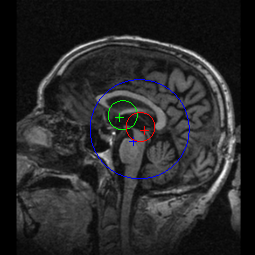
\includegraphics[scale=1.0]{v1_ACPC_sagittal.png}
\caption{v1\_ACPC\_sagittal.png shows the automatically detected MSP, the AC (green +), the PC (red +) and
the VSPS (blue +).  The circles show the search radii for the corresponding landmarks.  The search radii
can be changes using the -rac, -rpc and -rvsps options described above.
}
\label{fig:sagittal}
\end{center}
\end{figure}

The v1\_ACPC\_axial.png image (Figure \ref{fig:axial}) shows a tilt-corrected axial slice through the AC-PC.
Finally, v1\_orion.png (Figure \ref{fig:orion}) shows the 8 automatically detected Orion landmarks on the
MSP.  The $(i,j,k)$ coordinates of the Orion landmarks on the input volume are saved in v1\_orion.txt.

It is strongly recommended that the *png image be viewed to ensure that the automatics MSP, AC, PC and VSPS 
detections were successful.  If there is a failure in this process, the AC, PC and VSPS landmarks can be
manually supplied to the program  using the -lm argument. 
\vspace{3mm}

\begin{figure}
\begin{center}
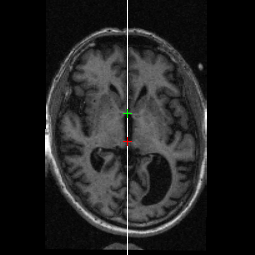
\includegraphics[scale=1.0]{v1_ACPC_axial.png}
\caption{v1\_ACPC\_axial.png shows the automatically detected MSP, the AC (green +), the PC (red +).
}
\label{fig:axial}
\end{center}
\end{figure}

\begin{figure}
\begin{center}
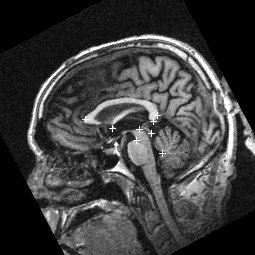
\includegraphics[scale=1.0]{v1_orion.png}
\caption{v1\_orion.png shows the 8 automatically Orion landmarks on the pitch-corrected MSP.
}
\label{fig:orion}
\end{center}
\end{figure}

\noindent {\large \bf Example 2:} In this example we customize the size and orientation of
the tilt-corrected output volume as follows:

acpcdetect -i \$ARTHOME/example1/v1.nii -v -nx 255 -ny 255 -nz 189 -dx 1.0 -dy 1.0 -dz 1.0 

-output-orient PIL

\noindent {In this case, the program prints out the following:}

Input image: /Users/ardekb01/babak\_lib/example1/v1.nii

Input image orientation: ASL

Input image matrix size: 256 x 256 x 128

Input image voxel size: 1.0000 x 1.0000 x 1.2500

Output image: /Users/ardekb01/babak\_lib/example1/v1\_PIL.nii

Output image matrix size: 255 x 255 x 189 

Output image voxel size: 1.0000 x 1.0000 x 1.0000

Output image orientation: PIL

Output transformation matrix: /Users/ardekb01/babak\_lib/example1/v1.mrx

Output transformation matrix (FSL format): /Users/ardekb01/babak\_lib/example1/v1\_FSL.mat 

\noindent Note that is this example the program printout changes to reflect the customized output volume dimensions
and orientation.  Incidentally, the custom dimensions specified in this example match those of
the volume \$ARTHOME/PILbrain.nii which represents the frequency that, after tilt-correction using
{\it acpcdetect}, an $(i,j,k)$ voxel coincides with intra-cranial space \citep{pmid35288224}. 
This can be used to quickly determine a good estimate of the intra-cranial region on the input volume
which may be useful in different applications \citep{pmid35288224}.
\vspace{3mm}

\noindent {\large \bf Example 3:} Occasionally the automatic detection of MSP, AC, PC and/or VSPS
fails. Failures would be apparent by viewing the *.png images.
Such is a case for volume \$ARTHOME/example2/v1.nii.  In these cases, the $(i,j,k)$ coordinates
of the AC, PC and VSPS landmarks on the input volume must be supplied to the program manually.  I recommend
using the AFNI software for manual identification of these landmarks. A video instruction for this 
can be found here: 

https://www.youtube.com/watch?v=q5GBaNnjOa8 

\noindent The manually identified landmarks are supplied to {\it acpcdetect} using the -lm argument.  For 
\$ARTHOME/example2/v1.nii we have found these landmarks and saved them in \\
\$ARTHOME/example2/v1.lm.  The {\it acpcdetect} program can then be run as follows:

acpcdetect -i \$ARTHOME/example2/v1.nii -lm \$ARTHOME/example2/v1.lm -v

\noindent {The program prints the following:}

Input image: /Users/ardekb01/babak\_lib/example2/v1.nii

Input image orientation: ASL

Input image matrix size: 256 x 256 x 128

Input image voxel size: 1.0000 x 1.0000 x 1.2500

Output image: /Users/ardekb01/babak\_lib/example2/v1\_RAS.nii

Output image matrix size: 128 x 256 x 256

Output image voxel size: 1.2500 x 1.0000 x 1.0000

Output image orientation: RAS

Manually specified landmarks: /Users/ardekb01/babak\_lib/example2/v1.lm

Output transformation matrix: /Users/ardekb01/babak\_lib/example2/v1.mrx

Output transformation matrix (FSL format): /Users/ardekb01/babak\_lib/example2/v1\_FSL.mat 

\noindent Note that the printout indicates the use of manually specified landmarks.
\bibliography{references}

\end{document}
